% #######################################
% ########### FILL THESE IN #############
% #######################################
\def\mytitle{COURSEWORK 1 REPORT}
\def\mykeywords{HTML, CSS, WebTech, Coursework}
\def\myauthor{Max Hodgso}
\def\contact{40274665@napier.ac.uk}
\def\mymodule{Web Technology (SET08101)}
% #######################################
% #### YOU DON'T NEED TO TOUCH BELOW ####
% #######################################
\documentclass[10pt, a4paper]{article}
\usepackage[a4paper,outer=1.5cm,inner=1.5cm,top=1.75cm,bottom=1.5cm]{geometry}
\twocolumn
\usepackage{graphicx}
\graphicspath{{./images/}}
%colour our links, remove weird boxes
\usepackage[colorlinks,linkcolor={black},citecolor={blue!80!black},urlcolor={blue!80!black}]{hyperref}
%Stop indentation on new paragraphs
\usepackage[parfill]{parskip}
%% Arial-like font
\IfFileExists{uarial.sty}
{
    \usepackage[english]{babel}
    \usepackage[T1]{fontenc}
    \usepackage{uarial}
    \renewcommand{\familydefault}{\sfdefault}
}{
    \GenericError{}{Couldn't find Arial font}{ you may need to install 'nonfree' fonts on your system}{}
    \usepackage{lmodern}
    \renewcommand*\familydefault{\sfdefault}
}
%Napier logo top right
\usepackage{watermark}
%Lorem Ipusm dolor please don't leave any in you final report ;)
\usepackage{lipsum}
\usepackage{xcolor}
\usepackage{listings}
%give us the Capital H that we all know and love
\usepackage{float}
%tone down the line spacing after section titles
\usepackage{titlesec}
%Cool maths printing
\usepackage{amsmath}
%PseudoCode
\usepackage{algorithm2e}

\titlespacing{\subsection}{0pt}{\parskip}{-3pt}
\titlespacing{\subsubsection}{0pt}{\parskip}{-\parskip}
\titlespacing{\paragraph}{0pt}{\parskip}{\parskip}
\newcommand{\figuremacro}[5]{
    \begin{figure}[#1]
        \centering
        \includegraphics[width=#5\columnwidth]{#2}
        \caption[#3]{\textbf{#3}#4}
        \label{fig:#2}
    \end{figure}
}

\lstset{
	escapeinside={/*@}{@*/}, language=C++,
	basicstyle=\fontsize{8.5}{12}\selectfont,
	numbers=left,numbersep=2pt,xleftmargin=2pt,frame=tb,
    columns=fullflexible,showstringspaces=false,tabsize=4,
    keepspaces=true,showtabs=false,showspaces=false,
    backgroundcolor=\color{white}, morekeywords={inline,public,
    class,private,protected,struct},captionpos=t,lineskip=-0.4em,
	aboveskip=10pt, extendedchars=true, breaklines=true,
	prebreak = \raisebox{0ex}[0ex][0ex]{\ensuremath{\hookleftarrow}},
	keywordstyle=\color[rgb]{0,0,1},
	commentstyle=\color[rgb]{0.133,0.545,0.133},
	stringstyle=\color[rgb]{0.627,0.126,0.941}
}

\thiswatermark{\centering \put(336.5,-38.0){\includegraphics[scale=0.8]{logo}} }
\title{\mytitle}
\author{\myauthor\hspace{1em}\\\contact\\Edinburgh Napier University\hspace{0.5em}-\hspace{0.5em}\mymodule}
\date{}
\hypersetup{pdfauthor=\myauthor,pdftitle=\mytitle,pdfkeywords=\mykeywords}
\sloppy
% #######################################
% ########### START FROM HERE ###########
% #######################################
\begin{document}
    \maketitle
    \begin{abstract}
        The following report outlines the process and details towards the creation of the calculator application
		for the Mobile application development.		
    \end{abstract}
    
    \textbf{Keywords -- }{\mykeywords}
    
    \section{Introduction}
	
	
    \paragraph{Referencing}
	\cite{https://www.androidauthority.com/build-a-calculator-app-721910/}
	\cite{www.w3schools.com}
	
	\Section{Software Design}
	For the design phase of this coursework, I created simple wire frames of some ideas to help get a better idea
	of what and how I wanted to implement.
	Ending up with a simple calculator as my final option not much was needed to be done my main focus in the design
	was to make sure that the layout of the calculator was user friendly and easy to interact with.
	
	\Section{Implementation}
	When implementing my website, the process was simple. 
	No aid was needed in the implementation of the user interface as previous experience in XML made this process smooth.
	The interface for the calculator consists of twelve buttons and a text view for input and output respectively.
	The buttons were made to be large and bold, for ease of use and to make it very easy for a user to see what they are doing, as the potential age demographic
	for this prototype can range from the very young to the very old.
	\includegraphics{calc.png}
	
	The background JavaScript for the calculator needed to import internal libraries that are pre-downloaded with Android Studio.
	These libraries allowed the buttons, text view and the grid layout in the user interface to used with the JavaScript.
	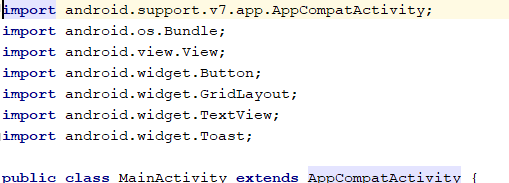
\includegraphics{Import.png}
	
	Finally, to catch errors, the toast operation was used in various places through out. This was used to prevent the use of two operators (+,/,-.*)
	being used within succession. If done so, the user is prompted of the error.
	Toast was also used for is the equals button is pressed when the user has not input a calculation, if done so this displays the number zero in the text view.
	
	\subsection{Toast}
	\begin{CodeEquals}
	            \else if(v.getId() == R.id.CalEquals){
                    \try {
                        double Result = Utility.evaluate(Output.getText().toString());
                        Output.setText(Double.toString(Result));
                    }
					
                    \catch(Exception e){
                        Toast.makeText(getApplicationContext(), e.getMessage(), Toast.LENGTH_LONG).show();
                        Output.setText("0");
                    }
                }
	\caption{Toast Equals}
	\end{CodeEquals}
	
	\begin{CodeOperator}
	                \else if(Output.getText().length() > 0 &&
                        Utility.isOperator(Output.getText().charAt(Output.getText().length() - 1)) &&
                        Utility.isOperator(buttonClicked.getText().charAt(0)))
						{
							String errorMessage = "You cannot enter two math operators in a row. You entered " + Output.getText().charAt(Output.getText().length() - 1) + " and " + buttonClicked.getText() + ".";
							Toast.makeText(getApplicationContext(), errorMessage, Toast.LENGTH_LONG).show();
						}

	\end{CodeOperator}
	
	\Section{Critical Evaluation}
	To begin, the application created, did keep with how I intended it to turn out, it kept a simplistic design and feel, which aimed to be user friendly and
	not be over complicated.
	The design was based around the basic calculators already found on mobiles and other devices (i.e: Computers)
	However, comparing already available similar applications, I feel I could have done more in terms of visual appeal.
	The colouring for the application are very bland and basic; although most users will not mind as most will just see it as a functional calculator, some 
	potential users (including myself) would appreciate some added visual appeal.
	Further more, adding some extra features may have been a nice bonus. The implementation process was already very simple and I should have added some extra time and effort
	into implementing more advanced calculations (Sin,binary-Decimal,%, etc.) that you can regularly find on most modern calculators.
	
	\subsection{Personal Evaluation}
	Reflecting on the creation of the coursework, the main challenges came from coding JavaScript. 
	This was only in the form of error catching, although 'toast' is the same as error catching I have used before, it was still a new concept to myself.
	However, I still feel more time and care should have been put towards this coursework.

	
	\section{Conclusion}
	In conclusion, the design and implementation of the mobile application, produced a basic and fully functional: Calculator application.
\bibliographystyle{ieeetr}
\bibliography{references}
		
\end{document}